%#!platex -kanji=utf8 hb.tex


%\advance \textheight -5.3zw


\color[cmyk]{0,0,0,.3}
\makeatletter
\long\def\makecaption#1#2{{\small
  \vskip \abovecaptionskip
  \sbox\@tempboxa{#1\relax #2}%
  \ifdim \wd\@tempboxa <\hsize \centering \fi
  \textcolor[cmyk]{0,0,0,.3}{#1\hskip1zw\relax #2}\par \nopagebreak
  \vskip .5\belowcaptionskip
  \nopagebreak
}}
\makeatother
\def\hoge#1#2{%
  \centering
  \bgroup
  \fboxsep=0pt%
  \fboxrule=.4pt%
%   \color[cmyk]{0,0,0,.3}\fbox
   {%
      \begin{minipage}{\linewidth}%
        \begin{center}%
          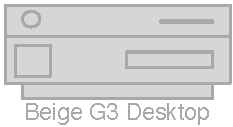
\includegraphics[height=1.5cm,clip]{gnu-head-above}\\
          \makecaption{図#1}{位置指定子に#2オプションを記述した画像}%
        \end{center}%
      \end{minipage}%
   }%
  \egroup
}

\begin{figure}[t]
 \hoge{1}{'t'}
\end{figure}

\begin{figure}[t]
 \hoge{2}{'t'}
\end{figure}

\Y{OTF}パッケージは\LaTeX で\W{Open Typeフォント}を扱うためのマクロパッ
ケージです.
\begin{figure}[h]
 \hoge{3}{'h'}
\end{figure}
\W{dviout}は制限付きで対応しています.単に\W{ユニコード}文字を使うためで
あれば\Y{UTF}パッケージを使えます.

\begin{figure}[b]
 \hoge{4}{'b'}
\end{figure}
